
\section{Overview} \label{sec:1.1}
\vspace{-0.5cm}
\noindent The alarming research interest in the field of digital signal processing (DSP) nowadays is due to improvements in digital circuit design and implementation \cite{deniz}. Adaptive filtering techniques are one of the well-known fields of DSP that has become prevalent and widely used in digital devices such as cell phones, digital cameras, medical instruments, etc. Unlike non-adaptive filters, the advantages of adaptive filters are their self-adjusting ability and iterative solution according to a certain optimization algorithm such least-mean-square (LMS) algorithm. As a result, adaptive filters have been applied to various fields such as control, communications, signal processing, etc., \cite{Haykins}, \cite{Hayes}.

\vspace{-0.5cm}
\par
\noindent Nowadays, the rapid emergence and use of hands-free telephones and internet phones have attracted a considerable research interest in echo cancellation as specific application of adaptive filtering techniques. An echo occurs in a communication system when an interruption and perhaps interfered versions of a signal are reproduced back to the sending end of that signal. This interruption version is only observable if the amount of the echo is substantially large \cite{son}. For instance, in the case of hands-free mobile communication, the acoustic coupling between headset and speaker phone may occasionally be strong enough to create echo to the extent that a user may seriously be irritated. And in internet phones such as skype or distance learning education via video-streaming, not just perfect data transmission is important, but better audio quality is also needed in these hypermedia role. For these reasons, effective echo cancellation is highly crucial to improve the audio quality and clarity of a call \cite{Gay}, \cite{Gilloire}. This requires adaptive filter to identify the echo path and efficiently cancel out the echo.

\vspace{-0.5cm}
\par
\noindent However, the nature of the echo path to be identified by the adaptive filter is sparse,and requires adaptive filters with sparsity exploitation property. Example of a sparse system that usually occurs in telecommunication networks is where a telephone equipment is connected to a packet switched network. In this case, the energy of the signal is typically of length 64-128ms, out of which the active region of the energy spans duration of 8-12ms, the remaining region is dominated by zero energy of the signal, making the impulse response sparse. The dominant portion is due to the presence of bulk delay caused by network propagation, encoding and jitter buffer delays \cite{Duttweiler}, \cite{Romesburg}, \cite{Benesty2}. Even though, sparse adaptive filters have been extensively studied for a long time to address the problem of echo in communication system. Up to date, the available filters fail to provide a tolerable performance due to challenging sparse nature of the echo path. For this particular application, where the system is sparse, conventional LMS filter performs poorly due to lack of sparsity exploitation property of the system. Hence, it is highly desirable to design a more efficient and robust adaptive filter that can provide acceptable performance for identifying sparse echo path. This can be achieved by exploiting the sparsity property of the systems \cite{Brookes}.

\vspace{-0.3cm}
%%%%%%%%%%%%%%%%%%%%%%%%%%%%%%%%%%%%%%%%%%%%%%%%%%%%%%%%%%%%%%%%%%%%%%
\section{The Aim of Adaptive Filter}\label{sec:1.2}
\vspace{-0.6cm}
\noindent In practical applications, an adaptive filter is employed to filter out a signal with an unknown  frequency response. Therefore, the main aim of an adaptive filter is to adjust its parameters to adapt with changes of system parameters \cite{shukur}. It does so by setting its parameters in such away that its output tries to minimize a meaningful objective function involving reference signal. In most cases, the objective function  is a function of the input, the reference and the adaptive filter output signal. An adaptive algorithm is composed of three basic items: definition of the minimization algorithm, definition of the objective function and definition of the error signal. The error signal is usually defined as the difference between the filter output and a desired response. The optimal filter parameters are found through minimization of a cost function of the error signal. A useful approach is based on minimizing the mean-square value of the error signal. The general configuration of an adaptive filtering system is shown in Fig. \ref{fig1x}. The input signal is denoted as $x(n)$, the output signal as $y(n)$, the desired response as $d(n)$ and the error signal as $e(n)=d(n)-y(n)$. The error signal is used to form a performance function that is iteratively minimized by the adaptation algorithm in order to determine the appropriate updating of the filter coefficients. The minimization of the objective function implies that the adaptive filter output signal matches the desired signal in some sense \cite{sayed}.
\begin{figure}[!htb]
\begin{center}
\vspace{1cm}
\epsfxsize = 10cm
\epsffile{Figures/Chapter1/fig1fir.eps}
%\includegraphics[width=70mm]{Fig1-TimesNewRomanPSMT.eps}
%\fbox{ \rule[-17mm]{0pt}{30mm} FIGURE }
\end{center}
\vspace{-1cm}
\caption{General Adaptive Filter Configuration, \cite{Haykins}.}
\label{fig1x}
\vspace{1.5cm}
\end{figure}

\vspace{-0.5cm}
\par
\noindent Basically, adaptive filters are classified into two major categories according to their impulse response, namely the finite impulse response (FIR); whose impulse response is of a finite duration because it settles to zero in finite time, and infinite impulse response (IIR) filters \cite{bellanger}; which have internal feedback and may continue to respond indefinitely. The most widely used filter is the FIR filter which will also be used throughout this work. Adaptive FIR filters have many structures such as adaptive transversal filters, the lattice predictor, the systolic array, etc. \cite{Haykins}. This adaptive transversal filters  structure is shown in Fig. \ref{fig2x}.

\vspace{-0.5cm}
\par
 \noindent From the figure, $\textbf{x}(n)$ denotes the tap input vector at time $n$, $\hat{d}(n|X_n)$ denotes the corresponding estimate of the desired response at the filter output, and $X_n$ denotes the space spanned by the tap inputs $x(n), x(n-1),\ldots, x(n-N+1)$. By comparing this with the actual desired response $d(n)$, then estimate error can be calculated as $e(n)=d(n)-\hat{d}(n|X_n)$.
 \begin{figure}[!htb]
\begin{center}
\vspace{1cm}
\epsfxsize = 14cm
\epsffile{Figures/Chapter1/fig2trans.eps}
%\includegraphics[width=70mm]{Fig1-TimesNewRomanPSMT.eps}
%\fbox{ \rule[-17mm]{0pt}{30mm} FIGURE }
\end{center}
\vspace{-1cm}
\caption{Structure of Adaptive Transversal Filter, \cite{shukur}.}
\label{fig2x}
\vspace{1.5cm}
\end{figure}


\vspace{-0.3cm}
%%%%%%%%%%%%%%%%%%%%%%%%%%%%%%%%%%%%%%%%%%%%%%%%%%%%%%%%%%%%%%%%%%%%%%
\section{Application of Adaptive filters}\label{sec:1.3}
\vspace{-0.5cm}
\noindent As previously discussed, an adaptive filter has the ability to self-adjust itself to operate well in an unknown environment and track variations of input signal statistics. These features make it a powerful device in many signal processing and control applications. Although, the nature of its applications differ in various aspects but have a common feature: the input signal and a desired response, which are used to estimate the error signal. Depending on the way the desired response is extracted, the applications of an adaptive filter can be classified into four categories: System identification, noise cancellation, channel equalization and linear prediction \cite{Haykins}. The configuration of each class will be briefly explained.



\vspace{-0.3cm}
%%%%%%%%%%%%%%%%%%%%%%%%%%%%%%%%%%%%%%%%%%%%%%%%%%%%%%%%%%%%%%%%%%%%%%
\subsection{Adaptive System Identification}\label{sec:1.3.1}
\vspace{-0.5cm}
\noindent  The adaptive system identification is basically used to estimate a transfer function of an unknown system such as the response of an unknown communication channel or the frequency response of an auditorium. In this case, the desired signal $d(n)$ is the output of an unknown system $u(n)$ when excited by the input signal $x(n)$. Both the the unknown system and the adaptive filter are driven by a common input $x(n)$ as shown in Fig. \ref{fig3x}. The output of the adaptive filter $y(n)$ is subtracted from the output of the unknown system resulting in an error estimate $e(n)$. The error is used to control the filter coefficients of the adaptive system. When the error signal is minimized, the adaptive filter represents the model for the unknown system \cite{Mathews}.

\begin{figure}[h]
\begin{center}
\vspace{1cm}
\epsfxsize = 10cm
\epsffile{Figures/Chapter1/fig4si.eps}
%\includegraphics[width=70mm]{Fig1-TimesNewRomanPSMT.eps}
%\fbox{ \rule[-17mm]{0pt}{30mm} FIGURE }
\end{center}
\vspace{-1cm}
\caption{Adaptive System Identification Configuration, \cite{shukur}.}
\label{fig3x}
\vspace{1.5cm}
\end{figure}

\vspace{-0.3cm}
%%%%%%%%%%%%%%%%%%%%%%%%%%%%%%%%%%%%%%%%%%%%%%%%%%%%%%%%%%%%%%%%%%%%%%
\subsection{Adaptive Noise Cancellation}\label{sec:1.3.2}
\vspace{-0.5cm}
\noindent In noise cancellation, adaptive filters let you remove noise from a signal in real time application. The adaptive noise cancellation configuration is illustrated in Fig. \ref{fig4x}. The signal of interest $s(n)$ is corrupted with uncorrelated additive noise $N_0(n)$, the combined signal is then used as the desired response $d(n)$  and is compared with the reference signal $x(n)$ that is uncorrelated with the noise signal $N_0(n)$ located at a different point. In this case, the adaptive filter provides an estimate $y(n)$ of the noise  $N_0(n)$, by exploiting the correlation between  $N_0(n)$ and  $N_1(n)$ so that the error signal will be a noiseless version of the target signal $s(n)$, \cite{shukur}, \cite{Glover}.

\begin{figure}[h]
\begin{center}
\vspace{1cm}
\epsfxsize = 10cm
\epsffile{Figures/Chapter1/fig5nc.eps}
%\includegraphics[width=70mm]{Fig1-TimesNewRomanPSMT.eps}
%\fbox{ \rule[-17mm]{0pt}{30mm} FIGURE }
\end{center}
\vspace{-1cm}
\caption{Adaptive Noise Cancellation Configuration, \cite{shukur}.}
\label{fig4x}
\vspace{1.5cm}
\end{figure}

\vspace{-0.3cm}
%%%%%%%%%%%%%%%%%%%%%%%%%%%%%%%%%%%%%%%%%%%%%%%%%%%%%%%%%%%%%%%%%%%%%%
\subsection{Adaptive Linear Prediction}\label{sec:1.3.3}
\vspace{-0.5cm}
\noindent In adaptive linear prediction application, the adaptive filter is used to estimate the values of a signal based on the past values of the signal. This application is essentially used in speech and image compression techniques. In this case, the desired signal $d(n)$ is a forward (or eventually backward) version of the adaptive filter input signal as shown in Fig. \ref{fig5x}. When the system converged, the adaptive filter represents a model  for the input signal and can used as a predictor model for the input signal \cite{Li}.

\begin{figure}[h]
\begin{center}
\vspace{1cm}
\epsfxsize = 10cm
\epsffile{Figures/Chapter1/fig7lp.eps}
%\includegraphics[width=70mm]{Fig1-TimesNewRomanPSMT.eps}
%\fbox{ \rule[-17mm]{0pt}{30mm} FIGURE }
\end{center}
\vspace{-1cm}
\caption{Adaptive Linear Prediction, \cite{shukur}.}
\label{fig5x}
\vspace{1.5cm}
\end{figure}



\vspace{-0.3cm}
%%%%%%%%%%%%%%%%%%%%%%%%%%%%%%%%%%%%%%%%%%%%%%%%%%%%%%%%%%%%%%%%%%%%%%
\subsection{Adaptive Channel Equalization}\label{sec:1.3.4}
\vspace{-0.5cm}
\noindent Channel equalization also known as inverse filtering consists of estimating a transfer function to compensate for the linear distortion caused by the channel due to spectral changes \cite{Chitre}, \cite{gui1}. For this case, the input signal $x(n)$ is applied through the unknown system $u(n)$ and then through the adaptive filter resulting in an output $y(n)$ as shown in Fig. \ref{fig6x}. The same input is also sent through a delay to attain $d(n)$. In this class of application, the adaptive system is said to be converged when the transfer function of the adaptive system is close to the reciprocal of the unknown system's transfer function.
\begin{figure}[!htb]
\begin{center}
\vspace{1cm}
\epsfxsize = 10cm
\epsffile{Figures/Chapter1/fig6ce.eps}
%\includegraphics[width=70mm]{Fig1-TimesNewRomanPSMT.eps}
%\fbox{ \rule[-17mm]{0pt}{30mm} FIGURE }
\end{center}
\vspace{-1cm}
\caption{Adaptive Channel Equalization Configuration, \cite{shukur}.}
\label{fig6x}
\vspace{1.5cm}
\end{figure}

% Therefore, the knowledge of sparse exploration is crucial for identification of such systems.
\vspace{-0.3cm}
%%%%%%%%%%%%%%%%%%%%%%%%%%%%%%%%%%%%%%%%%%%%%%%%%%%%%%%%%%%%%%%%%%%%%%
\section{Sparse Systems}\label{sec:1.4}
\vspace{-0.5cm}
\noindent A system is called sparse if its finite impulse response (FIR) model contains a few active taps in the presence of many negligible or zero ones \cite{Gay}, \cite{Douglas}. Sparse systems are classified into two main categories:
\vspace{-0.6cm}
\begin{itemize}
  \item General Sparse Systems: This consists a few active taps  interspersed among many negligible ones along the entire response of the system \cite{Hero}.
      \vspace{-0.3cm}
  \item Clustering Sparse Systems: This consists a cluster or gathering of large active taps at one or more positions along the response of the system \cite{Qing}.
      \vspace{-0.3cm}
\end{itemize}

\vspace{-0.3cm}
\par
\noindent A typical example of a single clustering sparse system is the acoustic echo path, while the echo path of a satellite links is an example of multi-clustering sparse system \cite{Gu1}. These systems are illustrated in Fig. \ref{fig7x}.

\begin{figure}[!htb]
\begin{center}
\vspace{1cm}
\epsfxsize = 10 cm
\epsffile{Figures/Chapter1/fig1ss.eps}
%\includegraphics[width=70mm]{Fig1-TimesNewRomanPSMT.eps}
%\fbox{ \rule[-17mm]{0pt}{30mm} FIGURE }
\end{center}
\vspace{-1cm}
\caption{Typical sparse system.}
\label{fig7x}
\end{figure}


%%%%%%%%%%%%%%%%%%%%%%%%%%%%%%%%%%%%%%%%%%%%%%%%%%%%%%%%%%%%%%%%%%%%%%
\section{Echo Cancellation}\label{sec:1.5}
\vspace{-0.5cm}
\noindent Even though echo cancellation has been studied for a long time and outstanding performance has been achieved by existing echo cancellers,
latest advances of hands-free telephony systems, internet phones such as VoIP or skype, and teleconferencing systems need additional
enhancement to increase the voice quality \cite{Christina}. In communication systems, an echo can be categorized into:

\vspace{-0.3cm}
\begin{enumerate} \vspace{-0.3cm}
\item Acoustic echo:  This is caused due to acoustic coupling between microphone and loudspeaker (e.g., as in speaker phone).

\vspace{-0.3cm}
\item Network echo: This occurs when there is an unbalanced coupling between 2-wire and 4-wire circuits.

\end{enumerate}
\vspace{-1cm}
\par
\noindent In both cases, the adaptive filter has to model an unknown system, i.e., the echo path. However, this thesis focuses on acoustic aspect of the echo. Fig. \ref{fig8x} illustrates a scenario of acoustic echo cancellation (AEC) configuration, where an adaptive filter is used to identify the unknown echo path by adaptively adjusting its coefficients. The estimated coefficients are used to provide a replica of the echoes which can be subtracted from the target signal to achieve cancellation.

%%%%%%%%%%%%%%%%%%%%%%%%%%%%%%%%%%%%%%%%%%%%%%%%%%%%%%%%%%%%%%%%%%%%%%%%%%%%%%%%%%%%
\vspace{-0.3cm}%%%%%%%%%%
%%%%%%%%%%%%%%%%%%%%%%%%%%%%%%%%%%%%%%%%%%%%%%%%%%%%%%%%%%%%%%%%%%
\subsection{Notations and Definitions}\label{sec:1.5.1}
\vspace{-0.5cm}
\begin{itemize}
\vspace{-0.3cm}
  \item $n$ is the discrete time index,
  \vspace{-0.3cm}
  \item $N$ is the length of the adaptive filter,
   \vspace{-0.3cm}
  \item $x(n)$ is the far-end signal (i.e., input signal of the adaptive filter and loudspeaker),
   \vspace{-0.3cm}
  \item $\textbf{x}(n)=[x(n), x(n-1),\ldots, x(n-N+1)]^T$ is the input tap vector,
  \vspace{-0.3cm}
  \item $\textbf{w}_0= [w_0,w_1,\ldots,w_{N-1}]^T$ is the impulse response of the system (i.e., the echo path).
  \vspace{-0.3cm}
  \item $\textbf{w}(n)=[w_0(n),w_1(n),\ldots,w_{N-1}(n)]^T$ is the estimated impulse response at time $n$ (i.e., the adaptive filter at time $n$,
  \vspace{-0.3cm}
  \item $y(n)=\textbf{w}_0^{T} \textbf{x}(n)$ is the echo signal,
  \vspace{-0.3cm}
  \item $\hat{y}(n)=\textbf{w}^{T}(n)\textbf{x}(n)$ is output of the adaptive filter,
  \vspace{-0.3cm}
  \item $d(n)=y(n)+v(n)$ is the reference signal or desired response.
  \vspace{-0.3cm}
\end{itemize}

\begin{figure}[!htb]
  \centering
  % Requires \usepackage{graphicx}
  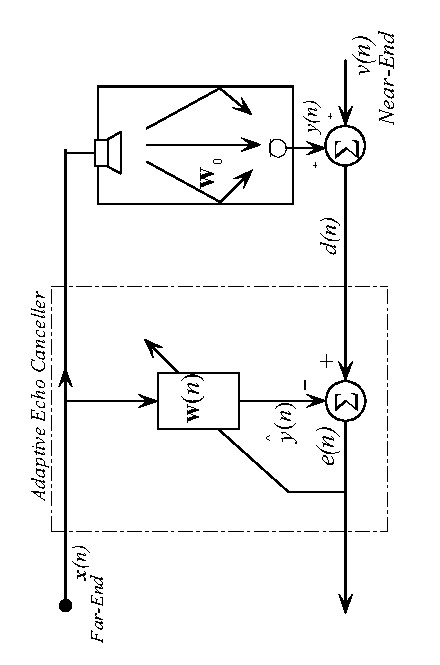
\includegraphics[width=8cm, angle=-90]{Figures/Chapter1/fig2path1.eps}\\
  \caption{Block diagram of acoustic room system.}
  \label{fig8x}
\end{figure}


\par
\vspace{-0.3cm}
\noindent Consider a loudspeaker and microphone in the same acoustic room. When the loudspeaker broadcast a signal $x(n)$, the microphone in the room will record the local signal $v(n)$ (i.e. near-end speech). In this case, the microphone signal to be transmitted back to the far-end side will be:

\vspace{-1.5cm}
%%%%%%%%%%%%%%%%%%%%%%%%%%%%%%%%%%%%%%%%%%%%%%%%%%%%%%%%%%%%%%%%%%%%%%
\begin{eqnarray}
\nonumber
d(n)&=&y(n)+v(n)\\
&=&\textbf{w}_0^{T} \textbf{x}(n)+v(n).\label{eq1a}
\end{eqnarray}
%%%%%%%%%%%%%%%%%%%%%%%%%%%%%%%%%%%%%%%%%%%%%%%%%%%%%%%%%%%%%%%%%%%%%%

\vspace{-0.6cm}
\par
\noindent If the echo path transfer function is modelled as FIR filter $\textbf{w}_{0}$, then the echo signal can be considered as filtered
 version of the loudspeaker signal i.e., $y(n)=\textbf{w}_{0}^T\textbf{x}(n)$ and the estimated output from the adaptive filter
 is $\hat{y}(n)=\textbf{w}^{T}(n)\textbf{x}(n)$. The function of the AEC in this case is to identify the unknown room impulse response $\textbf{w}_{0}$ and hence subtract an estimate of the echo signal from the microphone signal. Hence, the error signal is,

 \vspace{-1.5cm}
 %%%%%%%%%%%%%%%%%%%%%%%%%%%%%%%%%%%%%%%
 \begin{eqnarray}
 \nonumber
 e(n)&=&d(n)-\textbf{w}^T(n)\textbf{x}(n)\\
 &=&[\textbf{w}_0^{T}-\textbf{w}^{T}(n)] x(n)+v(n),\label{eq2a}
 \end{eqnarray}

 \vspace{-0.6cm}
 \noindent where $\textbf{w}(n)$ is an estimate of $\textbf{w}_{0}$. When the error signal is minimized, the adaptive filter estimate $\textbf{w}(n)$
 represents the echo path transfer function $\textbf{w}_{0}$ and therefore converges \cite{Elko}, \cite{Peterson}.


\vspace{-0.3cm}
\section{Performance Measures}\label{sec:1.6}
\vspace{-0.5cm}
\noindent Evaluation of performance measures influences the choice of one algorithm among many others. In echo cancellation problem, the aim is to measure how much the undesired echo is attenuated. There are many ways to measure this attenuation but the most important ones which are commonly adopted in this context would next be explained.

\vspace{-0.3cm}
%%%%%%%%%%%%%%%%%%%%%%%%%%%%%%%%%%%%%%%%%%%%%%%%%%%%%%%%%%%%%%%%%%%%%%
\subsection{Convergence Rate} \label{sec:1.6.1}
\vspace{-0.5cm}
\noindent This metric indicates the speed at which the filter converges to its steady state. A faster convergence rate is an efficient property of an adaptive filter. Usually, there is a trade-off between the convergence rate and other performance measures.

\vspace{-0.3cm}
%%%%%%%%%%%%%%%%%%%%%%%%%%%%%%%%%%%%%%%%%%%%%%%%%%%%%%%%%%%%%%%%%%%%%%
\subsection{Mean-Square-Error} \label{sec:1.6.2}
\vspace{-0.5cm}
\noindent The mean-square-error (MSE) is the mean square value of the difference between the desired signal and the filter output. An adaptive system has effectively converged to the true solution of the system if the MSE value is very small. It is given by:


%%%%%%%%%%%%%%%%%%%%%%%%%%%%%%%%%%%%%%%
\vspace{-1.5cm}
\begin{equation}
MSE=\mathrm{E}\{[d(n)-\hat{y}(n))]^2\},\label{eq3a}
\end{equation}

%%%%%%%%%%%%%%%%%%%%%%%%%%%%%%%%%%%%%%%%%%%%%%%%%%%%%%%%%%%%%%%%%%%%%%
\vspace{-0.6cm}
\noindent where $\mathrm{E}\{\cdot\}$ denotes expected value \cite{Mathews}.

\vspace{-0.3cm}
%%%%%%%%%%%%%%%%%%%%%%%%%%%%%%%%%%%%%%%%%%%%%%%%%%%%%%%%%%%%%%%%%%%%%%
\subsection{Mean-Square-Deviation} \label{sec:1.6.3}
\vspace{-0.5cm}
\noindent Mean-square-deviation (MSD) is the most used performance measure in echo cancellation. It quantifies directly how well an adaptive filter converges to the impulse response of the system that need to be identified. The MSD is defined as:

\vspace{-1.5cm}
%%%%%%%%%%%%%%%%%%%%%%%%%%%%%%%%%%%%%%%%%%%%%%%%%%%%%%%%%%%%%%%%%%%%%%
\begin{equation}
MSD=\mathrm{E}\|\textbf{w}_0-\textbf{w}(n)\|^{2}, \label{eq4a}
\end{equation}

\vspace{-0.6cm}
\noindent where $\|\cdot\|^2$ is the $l_2$-norm. It measures the closeness of an estimated system to that of the true system and is particulary useful to study the tracking capability of a time-varying system \cite{Dohono}.














































